\chapter{Event selection}\label{chap:event_sel}
\section{Good Run Lists}
Events to be analyzed must be present on the good run lists (GRLs) as defined by Table~\ref{tab:GRLs}. Listed luminosities of the samples were determined using Lumicalc (OflLumi-Run3-005) for $\pprefMBtrig$. In addition, event selection requires no error codes from the LAr, SCT, and Tile systems. Finally, events with noise bursts are rejected.

\begin{table}[!h]
\begin{center}
\begin{tabular}{c|c|c}
data sample & GRL & $\mathcal{L} [\inb]$ \\ \hline
$\pprefSample$  & $\mathrm{physics\_2024ppRef\_25ns.xml}$ & 7.75 \\
$\OOSample$  & GRLname.xml \\

$\NeNeSample$  & GRLname.xml \\
\end{tabular}
\end{center}
\caption{Table of the GRLs used}
\label{tab:GRLs}
\end{table}


\section{$\pprefSample$ data}

For pile-up (PU) effects studies, leveled subsets of low-$\mu$ and high-$\mu$ present in the run 488573 were selected. Otherwise, the full sample following the GRL file listed in the Table~\ref{tab:GRLs} is used for the analysis. LBs present both on the GRL and having a low-$\mu$ and high-$\mu$ setup are in Table~\ref{tab:PU_samples}.

\begin{table}[!h]
\begin{center}
\begin{tabular}{c|c|c|c|c}
sample & LB range & $\left\langle \mu \right\rangle$ & \# trig. events [M] & $\mathcal{L} [\mu \mathrm{b^{-1}}]$  \\ \hline
low-$\mu$ & 1433-1436; 1438-1509; 1512-1554; 1556-1585 & 0.2 & 1.07  & 20.8 \\
high-$\mu$ & 95-421; 424-599 & 4.0 & 11.9 &  724  \\
\end{tabular}
\end{center}
\caption{Low-$\mu$ and high-$\mu$ present in run 488573 sample statistics}
\label{tab:PU_samples}
\end{table}

\section{$\OOSample$ and $\NeNeSample$ data}
{\blue Selection should follow the one in the $\pprefSample$. When available, samples will be listed. }

\section{Gap cut}
Previous ATLAS measurement \cite{chargedHadroninPP2010} shows a non-negligible single diffractive (SD) contribution to the overall \pT spectrum. One way to suppress the SD contribution is to use gap analysis following the ATLAS study of pseudorapidity distribution of various diffraction modes \cite{gapXS}. Based on the listed publication, the gap cut is set at $\forwardgap = 3.5$. On Figure~\ref{fig:forward_gap} 
\begin{figure}[h]
    \centering
    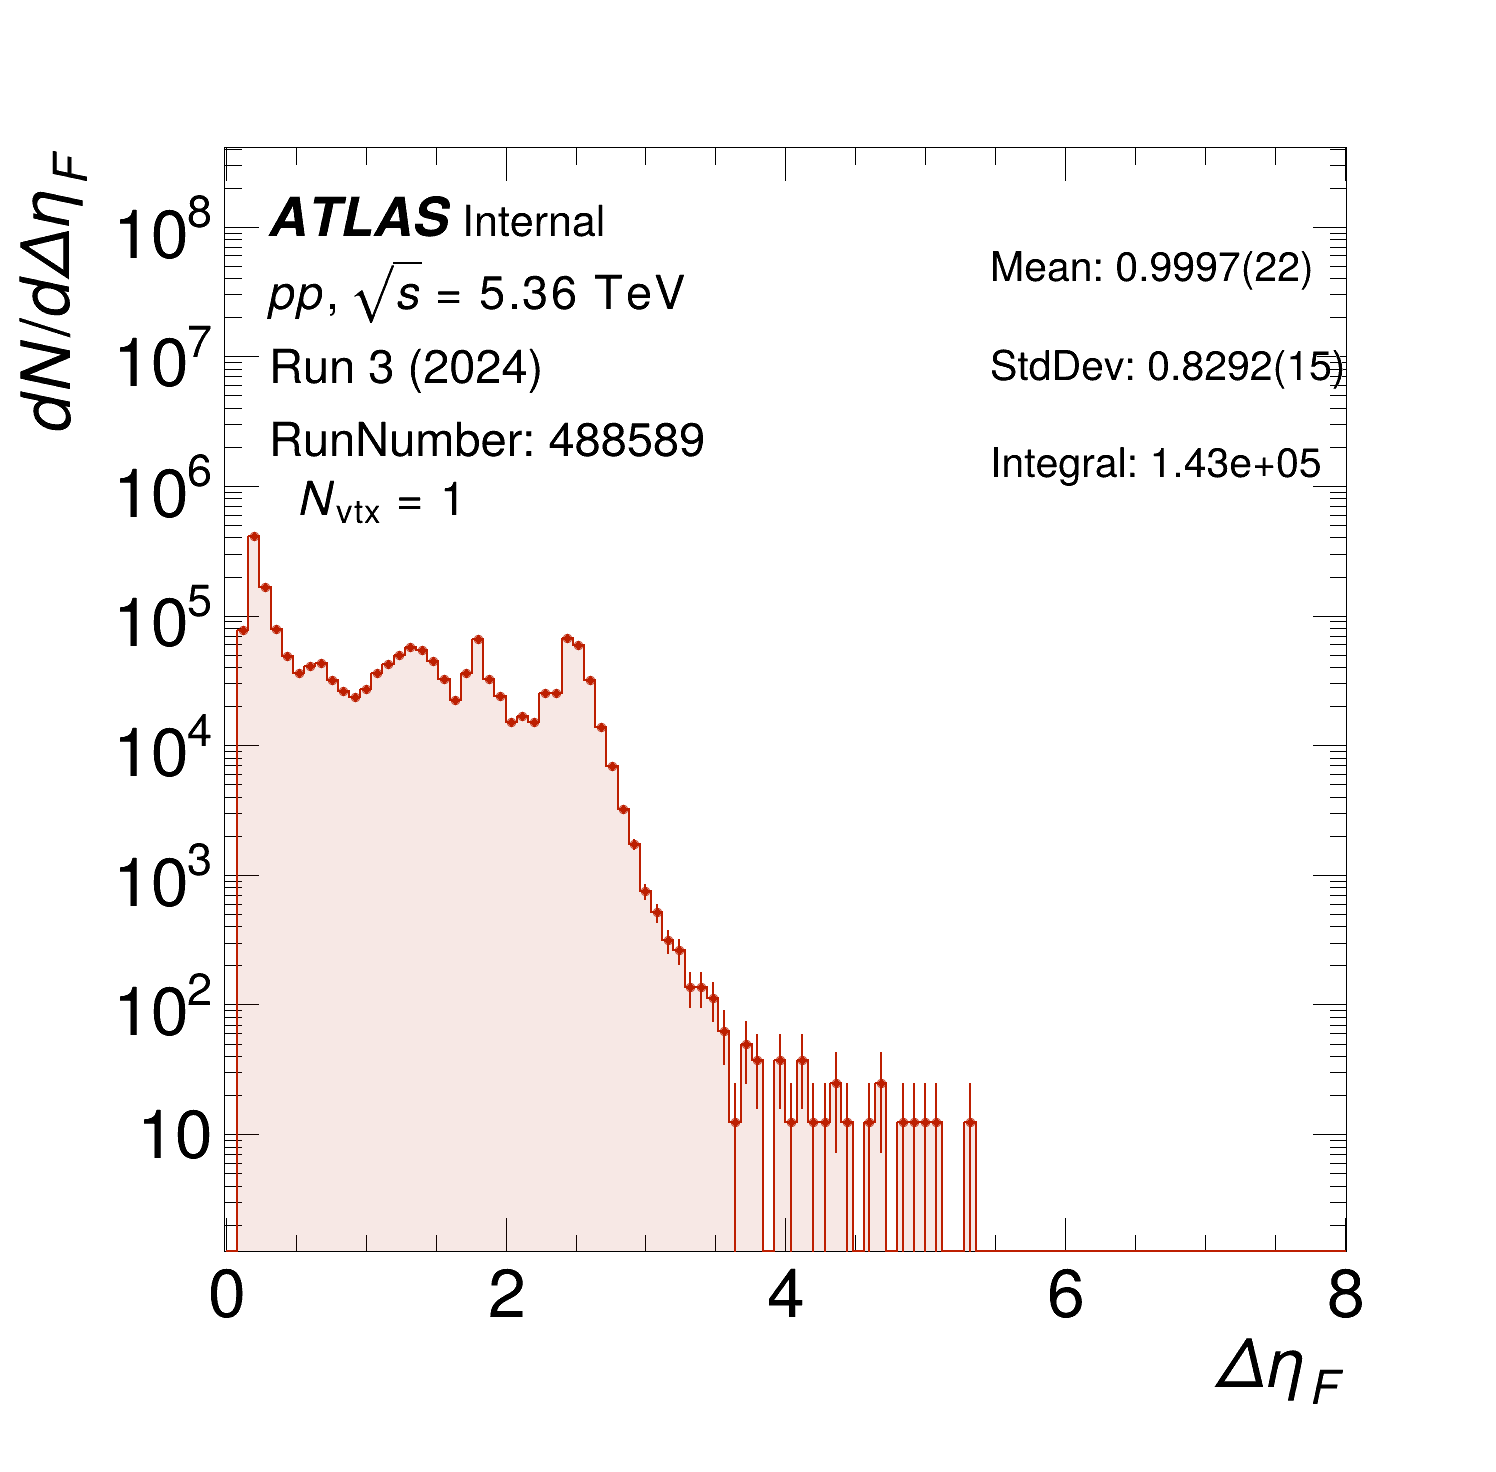
\includegraphics[width=0.7\linewidth]{images/forward_gap_488589.png}
    % 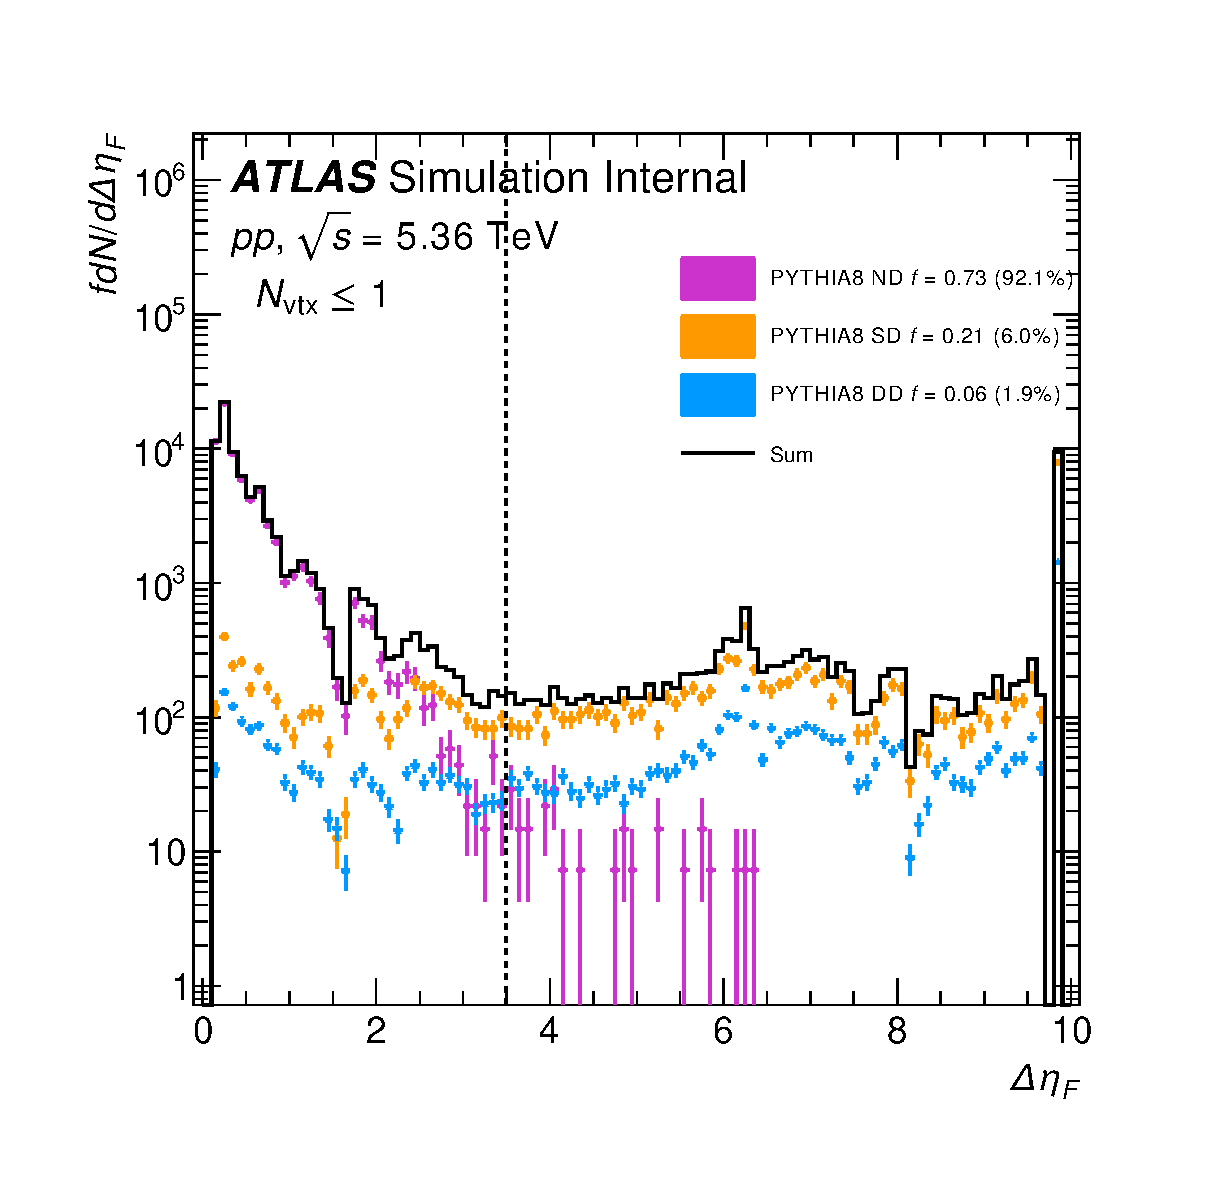
\includegraphics[width=0.7\linewidth]{images/rap_fwd_gap.eps}
    \caption{Forward gap $\forwardgap$ distribution for events with $N_\text{vtx} = 1$}
    \label{fig:forward_gap}
\end{figure} The distribution of $\forwardgap$ is shown in a subset of $\pprefSample$ data sample, where one can see that the number of events with $\forwardgap > 3.5$ is negligible. Events in that range are dominated by SD and DD processes. Since most of $\pprefSample$ was taken at $\mu\sim 4.0$, this creates another obstacle in resolving SD and DD events. Using the pilot production of no pile-up Pythia 8 samples, distributions for various diffraction modes were studied. Each mode got a weight corresponding to the ratio of cross-sections of the given processes, interpolated between $\sqn$ = 2.76 and 7 TeV, and normalized to get weight \cite{Ciesielski:2012mc}. The weights are listed in Table \ref{tab:diff_modes}.

\begin{table}[h]
    \centering
    \caption{The fraction of the various diffraction modes at $\sqn$ = 5.36 TeV; interpolated from \cite{Ciesielski:2012mc}}
    \begin{tabular}{c|c}
    Diffraction mode & Fraction \\
    \hline
    ND & $70.7\%$ \\
    SD & $15.7\%$ \\
    DD & $12.4\%$ \\
    CD & $1.2\%$ \\
    \end{tabular}
    \label{tab:diff_modes}
\end{table}

The Figure~\ref{fig:trigger_diffraction modes} shows the distribution of $\forwardgap$ in events, which fired an emulated $\pprefMBtrig$ trigger and have exactly one vertex. 
%\begin{figure}[h]
%    \centering
 %   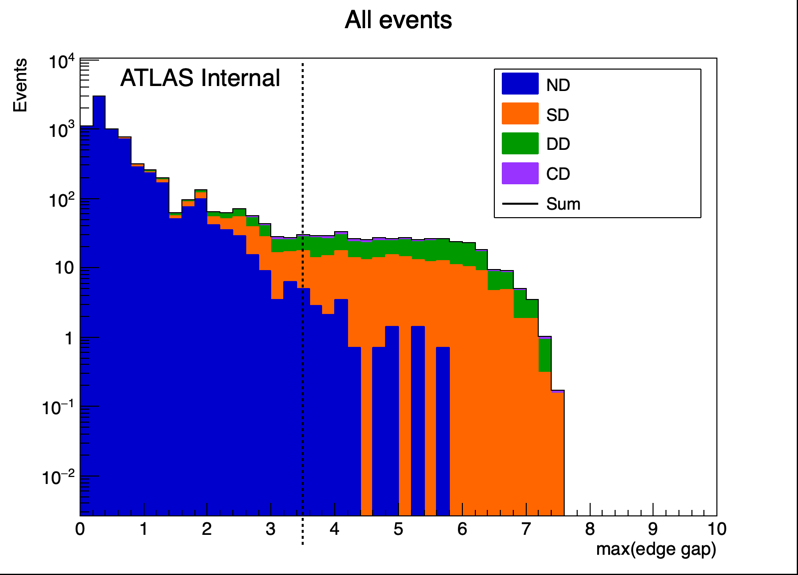
\includegraphics[width=0.6\linewidth]{images/gap_all_nv1.png}
 %   \caption{Forward gap $\forwardgap$ distribution for various diffraction modes in events with $N_\text{vtx} = 1$, all events}
  %  \label{fig:all_diffraction_modes}
%\end{figure}

\begin{figure}[h]
    \centering
    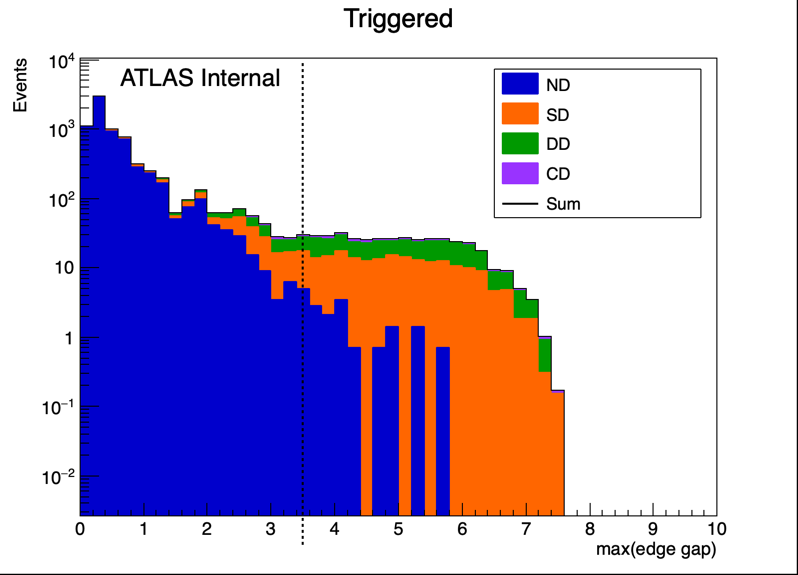
\includegraphics[width=0.7\linewidth]{images/gap_triggered_nv1.png}
    \caption{Forward gap $\forwardgap$ distribution for various diffraction modes in events with $N_\text{vtx} = 1$, mb\_sptrk trigger emulated events only}
    \label{fig:trigger_diffraction modes}
\end{figure}


One can notice that the cut at $\forwardgap > 3.5$ removes the majority of the single diffractive events. The fraction of single diffractive events with $\forwardgap < 3.5$ accounts for less than 4.4 \% of the events. 

\blue{The gap cut is not used so far in the final selection till this study concludes. To be studied further with full PYTHIA 8 production.} \black{} 